\documentclass[11pt,psfig]{article}
\usepackage{epsfig}
\usepackage{times}
\usepackage{amssymb}
\usepackage{float}

\newcount\refno\refno=1
\def\ref{\the\refno \global\advance\refno by 1}
\def\ux{\underline{x}}
\def\uw{\underline{w}}
\def\bw{\underline{w}}
\def\ut{\underline{\theta}}
\def\umu{\underline{\mu}} 
\def\bmu{\underline{\mu}} 
\def\be{p_e^*}
\newcount\eqnumber\eqnumber=1
\def\eq{\the \eqnumber \global\advance\eqnumber by 1}
\def\eqs{\eq}
\def\eqn{\eqno(\eq)}

 \pagestyle{empty}
\def\baselinestretch{1.1}
\topmargin1in \headsep0.3in
\topmargin0in \oddsidemargin0in \textwidth6.5in \textheight8.5in
\begin{document}
\setlength{\parskip}{1.2ex plus0.3ex minus 0.3ex}


\thispagestyle{empty} \pagestyle{myheadings} \markright{Homework
6: CS 274A, Probabilistic Learning: Winter 2014}



\title{CS 274A Homework 6}
\author{Probabilistic Learning: Theory and Algorithms, CS 274A, Winter 2014}
\date{Due Date: Wednesday March 12th in class}

\maketitle

\vfill\eject


\subsection*{Problem \ref: (10 points)}
Consider a classification problem with 2 classes and a single real-valued feature vector $X$, where class 1 has a Gaussian density $p(x|c_1)$ with parameters $\mu_1$ and $\sigma_1^2$, and class 2 has a Gaussian density $p(x|c_2)$ with parameters $\mu_2$ and $\sigma_2^2$.  
\begin{enumerate}
\item Derive a general expression for the location of the optimal decision regions as a function of the parameters.
\item Now assume $\mu_1 = 0$ and $\sigma_1^2 = 1$ and $\mu_2=3$ and $\sigma_2^2 = 3$. Also assume $p(c_1) = p(c_2) = 0.5$.  Draw or plot each of $p(x|c_1)p(c_1)$ and $p(x|c_2)p(c_2)$, as a function of $x$, on the same plot, clearly showing the optimal decision boundary (or boundaries).
\item Estimate the Bayes error rate for this problem within 3 decimal places of accuracy (you will need to use numerical tables for evaluating integrals of the Gaussian density function).
\item Answer parts 2 and 3 above but now with $p(c_1) = 0.9$.
    \end{enumerate}
You can use results/solutions from earlier homeworks if you wish.

Note that the Bayes error rate is defined as the minimum achievable (or optimal) classification error rate for a classification problem (assuming 0-1 loss). For two classes, in the general case it is defined as 
\[\int_{\ux}  \ \min\{P(c_1|\ux), 1 - P(c_1|\ux\} \ p(\ux) \ d\ux\]

\subsection*{Solution to Problem 1, Part 1}

Using Bayes rule we need to compute the following
\[
p(c_1|x) = \frac{p(x|c_1)p(c_1)}{p(x|c_1)p(c_1) + p(x|c_2)p(c_2)}
\]
Find when that is equal to 0.5 as that is the decision boundary. This occurs when
\[
\frac{1}{2} = \frac{1}{1 + \frac{p(x|c_2)p(c_2)}{p(x|c_1)p(c_1)}}
\]
It thus occurs when
\[
\frac{p(x|c_2)p(c_2)}{p(x|c_1)p(c_1)} = 1
\]
This is the same as
\[
\frac{p(x|c_2)}{p(x|c_1)} = \frac{p(c_1)}{p(c_2)}
\]
Let
\[
K_1 = \frac{1}{\sigma_1 \sqrt{2\pi}}
\]
\[
K_2 = \frac{1}{\sigma_2 \sqrt{2\pi}}
\]
\[
f_1(x) = \frac{(x-\mu_1)^2}{\sigma_1^2}
\]
\[
f_2(x) = \frac{(x-\mu_2)^2}{\sigma_2^2}
\]
We now have to solve the following
\[
\frac{K_2 \cdot e^{-f_2(x)/2}}{K_1 \cdot e^{-f_1(x)/2}} = \frac{p(c_1)}{p(c_2)}
\]
Let
\[
Q = \frac{p(c_1)K_1}{p(c_2)K_2} = \frac{p(c_1)\sigma_2}{p(c_2)\sigma_1}
\]
Then we have to solve the following
\[
\frac{e^{-f_2(x)/2}}{e^{-f_1(x)/2}} = Q
\]
\[
e^{f_1(x) - f_2(x)} = Q^2
\]
\[
f_1(x) - f_2(x) = 2 log(Q)
\]
\[
\frac{(x-\mu_1)^2}{\sigma_1^2} - \frac{(x-\mu_2)^2}{\sigma_2^2} = 2 log(Q)
\]
Let $S = 2 log(Q) \sigma_2^2 \sigma_1^2$ then it holds that
\[
\sigma_2^2(x-\mu_1)^2 - \sigma_1^2(x-\mu_2)^2 = S
\]
Expanding and then collecting terms together we get
\[
x^2(\sigma_1^2 - \sigma_2^2) + 2x(\mu_1 \sigma_2^2 - \mu_2 \sigma_1^2) + (\sigma_1^2 \mu_2^2 - \sigma_2^2 \mu_1^2 - S) = 0
\]
We now let
\[
a = \sigma_2^2 - \sigma_1^2
\]
\[
b = 2(\mu_2 \sigma_1^2 - \mu_1 \sigma_2^2)
\]
\[
c = \sigma_2^2 \mu_1^2 - \sigma_1^2 \mu_2^2 - S
\]
Then the solutions are the roots of the quadratic equation $ax^2 + bx + c = 0$ which are as follows
\[
x = \frac{-b \pm \sqrt{b^2 - 4ac}}{2a}
\]

\subsection*{Solution to Problem 1, Part 2}

For this problem we will be using
\[
p(x|c_1) = \frac{1}{\sqrt{2\pi}} e^{- \frac{x^2}{2}}
\]
\[
p(x|c_2) = \frac{1}{\sqrt{6\pi}} e^{- \frac{(x-3)^2}{6}}
\]
To get the decision boundaries we will solve the quadratic equation with
\[
a = 2
\]
\[
b = 6
\]
\[
Q = \sqrt{3}
\]
\[
S = 2 log(Q) 3 = 3log(3)
\]
\[
c = -9 - 3 log(3)
\]
After putting this all into Matlab, we end up with the following plot
\begin{figure}[H]
\centering
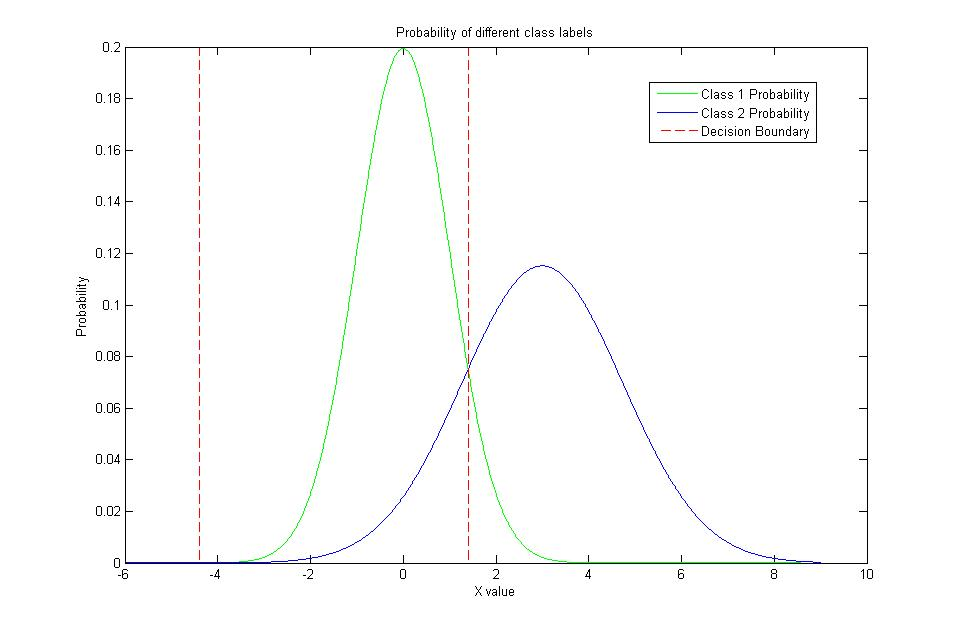
\includegraphics[height=5in]{prob1plot.jpg}
\caption{Probability of Class Labels with decision boundaries marked}
\end{figure}

\subsection*{Solution to Problem 1, Part 3}

For this case, if we let a and b be the decision boundaries and E be the error, then
\[
E = \int_{-\infty}^{a}{p(c_1|x)p(x) \, dx} + \int_{a}^{b}{p(c_2|x)p(x) \, dx} + \int_{a}^{\infty}{p(c_1|x)p(x) \, dx}
\]
For our case we can simplify this to
\[
E = \int_{-\infty}^{a}{p(x|c_1)p(c_1) \, dx} + \int_{a}^{b}{p(x|c_2)p(c_2) \, dx} + \int_{a}^{\infty}{p(x|c_1)p(c_1) \, dx}
\]
\[
E = 0.5(\int_{-\infty}^{a}{p(x|c_1) \, dx} + \int_{a}^{b}{p(x|c_2) \, dx} + \int_{a}^{\infty}{p(x|c_1) \, dx})
\]
For this case, according to the Matlab computation, we have $a=-4.3979$ and $b=1.3979$. \\
According to Wolfram Alpha
\[
\int_{-\infty}^{a}{p(x|c_1) \, dx} = \frac{1}{\sqrt{2\pi}} \int_{-\infty}^{-4.3979}{e^{-x^2/2} \, dx} = \frac{0.0000136991}{\sqrt{2\pi}} = 5.46515 \cdot 10^{-6}
\]
\[
\int_{a}^{b}{p(x|c_2) \, dx} = \frac{1}{\sqrt{6\pi}} \int_{-4.3979}^{1.3979}{e^{-(x-3)^2/6} \, dx} = \frac{0.77055}{\sqrt{6\pi}} = 0.177480
\]
\[
\int_{b}^{\infty}{p(x|c_1) \, dx} = \frac{1}{\sqrt{2\pi}} \int_{1.3979}^{\infty}{e^{-x^2/2} \, dx} = \frac{0.203216}{\sqrt{2\pi}} = 0.0810715
\]
Summing these three together we get the following estimate
\[
E = 0.1293
\]

\subsection*{Solution to Problem 1, Part 4}

To get the decision boundaries we will solve the quadratic equation with
\[
a = 2
\]
\[
b = 6
\]
\[
Q = 9 \sqrt{3}
\]
\[
S = 2 log(Q) 3 = 6 log(Q) = 6log( 9 \sqrt{3}) = 12 log(3) + 3 log(3) = 15 log(3)
\]
\[
c = -9 - 15 log(3)
\]
After putting this all into Matlab, we end up with the following plot
\begin{figure}[H]
\centering
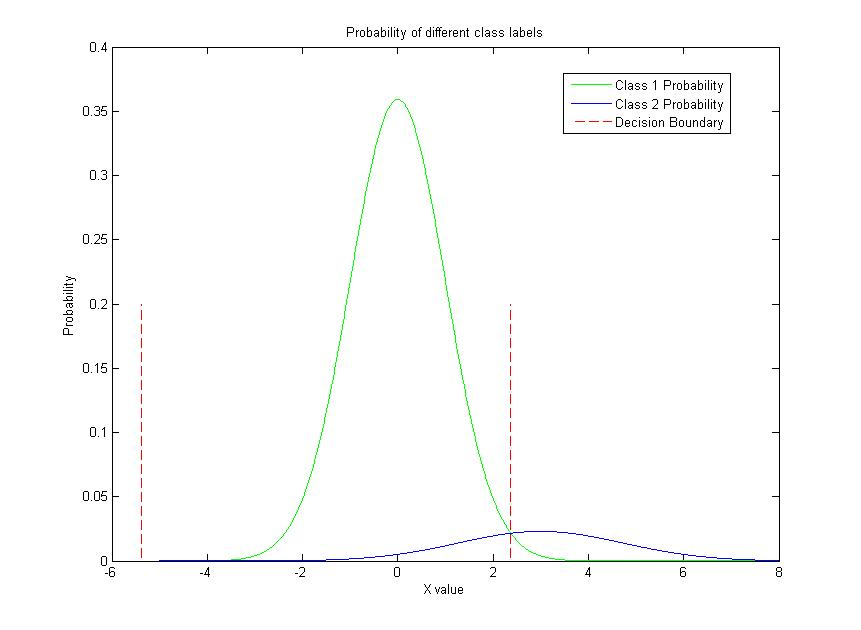
\includegraphics[height=5in]{prob1part2plot.jpg}
\caption{Probability of Class Labels with decision boundaries marked}
\end{figure}

For this case, if we let a and b be the decision boundaries and E be the error, then
\[
E = \int_{-\infty}^{a}{p(c_1|x)p(x) \, dx} + \int_{a}^{b}{p(c_2|x)p(x) \, dx} + \int_{a}^{\infty}{p(c_1|x)p(x) \, dx}
\]
For our case we can simplify this to
\[
E = \int_{-\infty}^{a}{p(x|c_1)p(c_1) \, dx} + \int_{a}^{b}{p(x|c_2)p(c_2) \, dx} + \int_{a}^{\infty}{p(x|c_1)p(c_1) \, dx}
\]
\[
E = 0.9\int_{-\infty}^{a}{p(x|c_1) \, dx} + 0.1\int_{a}^{b}{p(x|c_2) \, dx} + 0.9\int_{a}^{\infty}{p(x|c_1) \, dx}
\]
For this case, according to the Matlab computation, we have $a=-5.3716$ and $b=2.3716$. \\
According to Wolfram Alpha
\[
\int_{-\infty}^{a}{p(x|c_1) \, dx} = \frac{1}{\sqrt{2\pi}} \int_{-\infty}^{-5.3716}{e^{-x^2/2} \, dx} = \frac{9.781 \cdot 10^{-8}}{\sqrt{2\pi}} = 3.90205 \cdot 10^{-8}
\]
\[
\int_{a}^{b}{p(x|c_2) \, dx} = \frac{1}{\sqrt{6\pi}} \int_{-5.3716}^{2.3716}{e^{-(x-3)^2/6} \, dx} = \frac{1.55592}{\sqrt{6\pi}} = 0.358374
\]
\[
\int_{b}^{\infty}{p(x|c_1) \, dx} = \frac{1}{\sqrt{2\pi}} \int_{2.3716}^{\infty}{e^{-x^2/2} \, dx} = \frac{0.0221978}{\sqrt{2\pi}} = 0.00885564
\]
Summing these three together we get the following estimate
\[
E = 0.0438
\]


\subsection*{Problem \ref: (10 points)}

Consider a classification problem  with 2 classes and a single real-valued feature vector $X$.
For class 1, $p(x|c_1)$ is uniform $U(a,b)$  with $a=2$ and $b=4$. For class 2, $p(x|c_2)$ is exponential with density $\lambda \exp(-\lambda x)$ where $\lambda=1$. Let $p(c_1) = p(c_2) = 0.5$.
\begin{enumerate}
\item Determine the location of the optimal decision regions
\item Draw a sketch of the two class densities multiplied by $P(c_1)$ and $P(c_2)$ respectively, as a function of $x$, clearly showing the optimal decision boundary (or boundaries)
\item Compute the Bayes error rate for this problem within 3 decimal places of accuracy
    \item Answer the questions above but now with $a=2$ and $b=22$.
    \end{enumerate}
		
\subsection*{Solution to Problem 2}

From previous problem we have to solve
\[
\frac{p(x|c_2)}{p(x|c_1)} \leq \frac{p(c_1)}{p(c_2)}
\]
Given our values we have
\[
\frac{p(x|c_2)}{p(x|c_1)} \leq 1
\]
\[
p(x|c_2) \leq p(x|c_1)
\]
That is when it is optimal to choose $c_1$. This occurs when
\[
exp(-x) \leq 0.5
\]
\[
x \geq log(2)
\]
However, we can only choose $c_1$ for $2 \leq x \leq 4$. Our condition is satisfied in that region, thus the decision regions are as follows:

$c_1$ if $2 \leq x \leq 4$

$c_2$ otherwise

\subsection*{Solution to Problem 2, Part 2}

After putting this all into Matlab, we end up with the following plot
\begin{figure}[H]
\centering
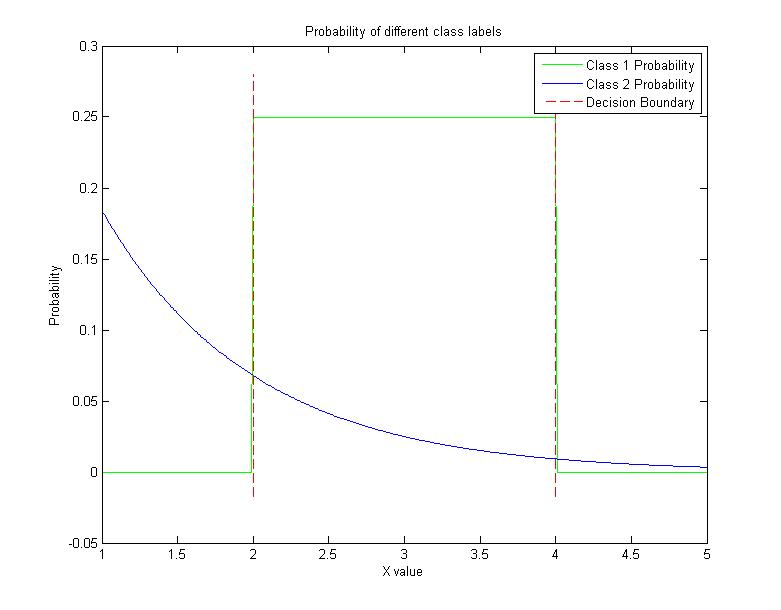
\includegraphics[height=5in]{prob2plot.jpg}
\caption{Probability of Class Labels with decision boundaries marked}
\end{figure}

\subsection*{Solution to Problem 2, Part 3}

For this case, if we let a and b be the decision boundaries and E be the error, then
\[
E = \int_{-\infty}^{a}{p(c_1|x)p(x) \, dx} + \int_{a}^{b}{p(c_2|x)p(x) \, dx} + \int_{a}^{\infty}{p(c_1|x)p(x) \, dx}
\]
For our case we can simplify this to
\[
E = \int_{-\infty}^{a}{p(x|c_1)p(c_1) \, dx} + \int_{a}^{b}{p(x|c_2)p(c_2) \, dx} + \int_{a}^{\infty}{p(x|c_1)p(c_1) \, dx}
\]
\[
E = 0.5\int_{-\infty}^{a}{p(x|c_1) \, dx} + 0.5\int_{a}^{b}{p(x|c_2) \, dx} + 0.5\int_{a}^{\infty}{p(x|c_1) \, dx}
\]
For this case we have $a=2$ and $b=4$. \\
\[
\int_{-\infty}^{a}{p(x|c_1) \, dx} = 0
\]
\[
\int_{a}^{b}{p(x|c_2) \, dx} = \int_{2}^{4}{e^{-x} \, dx} = e^{-2} - e^{-4} = 0.1170
\]
\[
\int_{b}^{\infty}{p(x|c_1) \, dx} = 0
\]
Summing these three together we get the following estimate
\[
E = 0.0585
\]

\subsection*{Problem \ref: (10 points)}

Consider a 2-class classification problem with $d$-dimensional real-valued inputs $\ux$, where the class-conditional densities, $p(\ux|c_1)$ and $p(\ux|c_2)$ are multivariate Gaussian with different means $\umu_1$ and $\umu_2$ and a common covariance matrix $\Sigma$, with class probabilities $P(c_1)$ and $P(c_2)$.
\begin{enumerate}
\item Write the discriminant functions for this problem in the form of
$g_1(\ux) = \log p(x|c_1) + \log p(c_1)$ (same for $g_2(\ux)$).
\item Prove that the optimal decision boundary, at $g(\ux) = g_1(\ux) - g_2(\ux) = 0$, can be written in the form of a linear discriminant, $\uw^t \ux + w_0 = 0$, where $\uw$ is a $d$-dimensional weight vector and $w_0$ is a scalar, and clearly indicate what $\uw$ and $w_0$ are in terms of the parameters of the classification model.
\item Show that if $P(c_1) = P(c_2)$ then the classifier can be viewed as a ``nearest mean" type of classifier, where a vector $\ux$ is assigned to the mean that it is closest to, and where distance is measured using Mahalanobis distance.
\end{enumerate}

\subsection*{Solution to Problem 3, Part 1}
First, we will let
\[
K = \frac{1}{(2\pi)^{d/2}|\Sigma|^{1/2}}
\]
\[
f_1(x) = (x-\mu_1)^T \Sigma^{-1} (x-\mu_1)
\]
\[
f_2(x) = (x-\mu_2)^T \Sigma^{-1} (x-\mu_2)
\]
then it holds that
\[
g_1(x) = log(K) - \frac{1}{2}f_1(x) + log(p(c_1))
\]
\[
g_1(x) = -log((2\pi)^{d/2} |\Sigma|^{1/2}) - \frac{1}{2}f_1(x) + log(p(c_1))
\]
\[
g_1(x) = -\frac{1}{2}( d \cdot log(2\pi) + log(|\Sigma|) + f_1(x)) + log(p(c_1))
\]
By the same token
\[
g_2(x) = -\frac{1}{2}( d \cdot log(2\pi) + log(|\Sigma|) + f_2(x)) + log(p(c_2))
\]

\subsection*{Solution to Problem 3, Part 2}

By some algebraic manipulation, it holds that
\[
g(x) = g_1(x)-g_2(x) = - \frac{1}{2} f_1(x) + \frac{1}{2} f_2(x) + log(p(c_1)) - log(p(c_2))
\]
\[
g(x) = \frac{1}{2} ( f_2(x) - f_1(x) ) + log(p(c_1)) - log(p(c_2))
\]
Let $v = -2( log(p(c_2)) - log(p(c_1)) )$ then we have to solve
\[
v = f_2(x) - f_1(x)
\]
\[
(x^T \Sigma - \mu_2^T \Sigma)(x - \mu_2) - (x^T \Sigma - \mu_1^T \Sigma)(x - \mu_1) = v
\]
\[
(x^T \Sigma x - \mu_2^T \Sigma x - x^T \Sigma \mu_2 + \mu_2^T \Sigma \mu_2) - (x^T \Sigma x - \mu_1^T \Sigma x - x^T \Sigma \mu_1 + \mu_1^T \Sigma \mu_1) = v
\]
Collecting terms we end up with
\[
(\mu_1^T \Sigma - \mu_2^T \Sigma) x + x^T (\Sigma \mu_1 - \Sigma \mu_2) + \mu_2^T \Sigma \mu_2 - \mu_1^T \Sigma \mu_1 = v
\]
If we let
\[
u = v - \mu_2^T \Sigma \mu_2 + \mu_1^T \Sigma \mu_1
\]
Then after some factoring we have
\[
(\mu_1^T - \mu_2^T) \Sigma x + x^T \Sigma (\mu_1 - \mu_2) = u
\]
If we let $\mu_0 = \mu_1 - \mu_2$ then we further have
\[
\mu_0 \Sigma x + x^T \Sigma \mu_0 = u
\]
If we let $m_1 = \mu_0 \Sigma$ and $m_2 = \Sigma \mu_0$ then we have
\[
m_1 x + x^T m_2 - u = 0
\]
This is the same as
\[
dot(m_1,x) + dot(m_2,x) - u = 0
\]
Thus we can further day that
\[
(m_1 + m_2^T)x - u = 0
\]
Thus finally let
\[
w = (m_1 + m_2^T)
\]
\[
w_0 = -u
\]
then we have the linear decision boundary

\subsection*{Solution to Problem 3, Part 3}

If $p(c_1) = p(c_2)$ then $v=0$ above, so we have
\[
f_1(x) = f_2(x)
\]
\[
(x-\mu_1)^T \Sigma (x-\mu_1) = (x-\mu_2)^T \Sigma (x-\mu_2)
\]
The decision boundary is thus when the two MH distances are equal so the class will end up taking on the value of whichever mean is closer. 

\subsection*{Problem \ref: (10 points)}
Consider the situation  in Problem 3, for the case of $d=2$ and $p(c_1) =
p(c_2)$, and with the mean of class 1  at $(1,1)$ and the mean of the second
class at $(4,4)$ and with a covariance matrix defined so that $\sigma_{11} =
1$, $\sigma_{22} = 4$, and $\sigma_{12} = 1$.  Draw or plot a figure in the
2-dimensional space ($x_1$, $x_2$) that shows  
\begin{enumerate}
%(a) probability contours for $p(\ux|c_i), i = 1, 2$, and (b) 
\item the location of the optimal
decision boundary relative to the two class means.  If you wish you can use
MATLAB to generate the plots for you, but hand-drawn is also fine.
\item the location of the optimal
decision boundary relative with $p(c_1) = 0.8, p(c_2) = 0.2$. Provide a
1-line interpretation of why the result is different to part 1.
\end{enumerate}

\subsection*{Solution to Problem 4, Part 1}

After doing some algebraic manipulation, solving it turns out to be solving
\[
(x-1)^2 + (x-1)(y-1) + (x-1)(y-1) + 4(y-1)^2 = (x-4)^2 + (x-4)(y-4) + (x-4)(y-4) + 4(y-4)^2
\]
After more manipulation
\[
(x-1)^2 + 2(x-1)(y-1) + 4(y-1)^2 = (x-4)^2 + 2(x-4)(y-4)+ 4(y-4)^2
\]
Expanding we get
\[
(x^2-2x+1) + 2(xy-x-y+1) + 4(y^2-2y+1) = (x^2-8x+16) + 2(xy-4x-4y+16)+ 4(y^2-8y+16)
\]
After some cancelling
\[
(-2x+1) + 2(-x-y+1) + 4(-2y+1) = (-8x+16) + 2(-4x-4y+16)+ 4(-8y+16)
\]
Expanding out again
\[
-2x+1 - 2x - 2y + 2 -8y + 4 = -8x+16 -8x-8y+32 -32y+64
\]
\[
-4x-10y+7 = -16x-40y+112
\]
\[
y = \frac{-12x+105}{30}
\]
\begin{figure}[H]
\centering
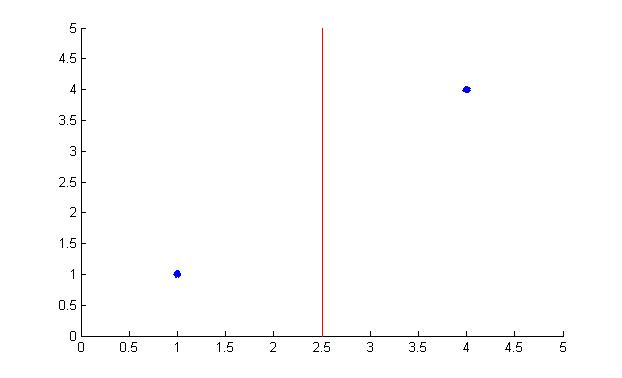
\includegraphics[height=3.25in]{plot4_part1.jpg}
\caption{The decision boundary with the means}
\end{figure}

\subsection*{Solution to Problem 4, Part 2}

After plugging in values, we end up with
\[
w = (-12,-30)
\]
\[
w_0 = 103.8
\]

\begin{figure}[H]
\centering
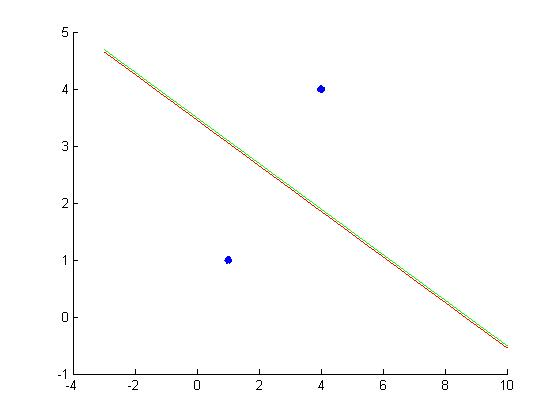
\includegraphics[height=3.25in]{plot4_part2.jpg}
\caption{The decision boundary with the means}
\end{figure}

\subsection*{Problem \ref: (10 points)}
Consider a 2 class problem with labeled training data $D = \{\ux_i, c_i\}$, where $c_i \in \{0,1\}$ and $i=1,\ldots,N$. Assume you are working with 2 different classification models $M_1$ and $M_2$ with parameters $\theta$ and $\phi$ respectively, where each model's functional form can be written as
$p(c | \ux, \hat{\theta})$ and $p(c | \ux, \hat{\phi})$ respectively, where
$\hat{\theta}$ and $\hat{\phi}$ are point estimates of the parameters. For example $M_1$ could be   a logistic regression model   and   $M_2$ could be a neural network with a single hidden layer---the details of these models are not important for this problem. Assume you are fully Bayesian in the way you wish to approach the problem.  How would you make classification decisions as a Bayesian, i.e., how would you decide whether the probability of one class or the other is more likely given a new test vector $\ux$?  (Hint: it may help to start by thinking about $p(c | \ux, D)$). Clearly explain all steps in your answer.

\subsection*{Solution to Problem 5}

First, you would figure out a probability on the class labels given the parameters of the model, so you need
\[
p(c|\hat{\theta})
\]
To figure out the class probability we will say that
\[
p(c|x,\hat{\theta}) = \frac{p(x|c,\hat{\theta})p(c|\hat{\theta})}{p(x)}
\]
By law of total probability, $p(x) = p(x|c,\hat{\phi}) + p(x|c,\hat{\theta})$. Thus we end up with
\[
p(c|x,\hat{\theta}) = \frac{p(x|c,\hat{\theta})p(c|\hat{\theta})}{p(x|c,\hat{\phi}) + p(x|c,\hat{\theta})}
\]
You do the same thing for $p(c|x,\hat{\phi})$ and figure out which probability is greater. 


\subsection*{Problem \ref: (10 points)}
In class we showed that least squares regression could be related to a conditional  Gaussian likelihood. Assume we have training data in the form  $D = \{x_i, y_i\}$, where $x$ and $y$ are both 1-dimensional and $i=1,\ldots,N$. Say we assume a model of the form $E[y] = a x + b$ with $y$ having Gaussian noise with variance $\sigma^2$ and mean $E[y]$. Derive maximum likelihood estimates for each of $a$, $b$, and $\sigma^2$.

\subsection*{Solution to Problem 6}

For this problem, we are assuming that at each pair of points, there is a Gaussian distribution for $y$ given $x$ where the mean $\mu_y = ax+b$ and the variance is $\sigma^2$.
\\
We will define $\theta=(a,b,\sigma)$, then
\[
L(D|\theta) = \prod_{i=1}^N{ \frac{1}{\sigma \sqrt{2\pi}} exp(-\frac{(y_i - (ax_i + b))^2}{2\sigma^2})}
\]
Taking the log to get log-likelihood we have
\[
l(\theta) = -\frac{N}{2} log(2\pi \sigma^2) + \sum_{i=1}^N{-\frac{(y_i - (ax_i + b))^2}{2\sigma^2}}
\]
Simplifying further we have
\[
l(\theta) = -\frac{N}{2} log(2\pi \sigma^2) - \frac{1}{2\sigma^2} \sum_{i=1}^N{(y_i - (ax_i + b))^2}
\]
Expanding out the square we have
\[
l(\theta) = -\frac{N}{2} log(2\pi \sigma^2) - \frac{1}{2\sigma^2} \sum_{i=1}^N{y_i^2 -2y_i (ax_i + b) + (ax_i + b)^2}
\]
Expanding out the square again
\[
l(\theta) = -\frac{N}{2} log(2\pi \sigma^2) - \frac{1}{2\sigma^2} \sum_{i=1}^N{[y_i^2 -2ay_i x_i -2by_i + a^2 x_i^2 + 2abx_i + b^2]}
\]
We will find $\hat{a}_{ML}$ and $\hat{b}_{ML}$ by first taking the partials
\[
\frac{\partial l}{\partial a} = - \frac{1}{2\sigma^2} \sum_{i=1}^N{[-2y_i x_i + 2a x_i^2 + 2bx_i]}
\]
\[
\frac{\partial l}{\partial b} = - \frac{1}{2\sigma^2} \sum_{i=1}^N{[-2y_i + 2a x_i + 2b]}
\]
Setting both equal to zero we end up having to solve the following equations
\[
\sum_{i=1}^N{[-y_i x_i + a x_i^2 + bx_i]} = 0
\]
\[
\sum_{i=1}^N{[-y_i + a x_i + b]} = 0
\]
Rearranging the sums and putting into a linear system form, we have the solve the following
\[
a\sum_{i=1}^N{x_i^2} + b\sum_{i=1}^N{x_i} = \sum_{i=1}^N{y_i x_i}
\]
\[
a\sum_{i=1}^N{x_i} + b \cdot N = \sum_{i=1}^N{y_i}
\]
For shorthand, we will now let
\[
A = \sum_{i=1}^N{x_i^2}
\]
\[
B = \sum_{i=1}^N{x_i}
\]
\[
C = \sum_{i=1}^N{y_i x_i}
\]
\[
D = \sum_{i=1}^N{y_i}
\]
Then we are left with solving
\[ \left( \begin{array}{ccc}
A & B \\
B & N \end{array} \right)
\left( \begin{array}{ccc}
a \\
b \end{array} \right)=
\left( \begin{array}{ccc}
C \\
D \end{array} \right)\]
After doing the matrix inverse, we have the following 
\[ 
\left( \begin{array}{ccc}
a \\
b \end{array} \right) =
\frac{1}{AN - B^2}
\left( \begin{array}{ccc}
N & -B \\
-B & A \end{array} \right)
\left( \begin{array}{ccc}
C \\
D \end{array} \right)
\]
Thus finally we can say that
\[
\hat{a}_{ML} = \frac{NC-BD}{AN-B^2}
\]
\[
\hat{b}_{ML} = \frac{AD-BC}{AN-B^2}
\]
We now want to find $\hat{\sigma^2}_{ML}$. If we let
\[
K = \sum_{i=1}^N{(y_i - (ax_i + b))^2}
\]
then we will have after letting $v = \sigma^2$
\[
l(\theta) = -\frac{N}{2} log(2\pi v) - \frac{K}{2v}
\]
Taking the derivative with respect to v we have
\[
l'(\theta) = -\frac{N}{2v} + \frac{K}{2v^2}
\]
Setting it equal to zero we have to solve
\[
Kv = N v^2
\]
We can assume a non-zero variance so we can assert that
\[
v = \frac{K}{N}
\]
Finally we can say that
\[
\hat{\sigma^2}_{ML} = \frac{1}{N} \sum_{i=1}^N{(y_i - (ax_i + b))^2}
\]
\end{document}








